\documentclass[10pt]{article}
\usepackage[letterpaper,margin=0.82in]{geometry}
\usepackage[T1]{fontenc}
\usepackage{lmodern}
\usepackage{microtype}
\usepackage{amsmath,amssymb,amsthm,mathtools}
\usepackage{booktabs,tabularx,array,longtable,multirow}
\usepackage{graphicx}
\usepackage{xcolor}
\usepackage{enumitem}
\usepackage{caption}
\usepackage{subcaption}
\usepackage{url}
\usepackage[hidelinks]{hyperref}
\usepackage{fancyhdr}
\usepackage{lastpage}
\usepackage{setspace}
\usepackage{placeins}

\definecolor{qrpblue}{HTML}{17365D}
\definecolor{qrpteal}{HTML}{226B75}
\definecolor{qrpgray}{HTML}{5D6570}
\definecolor{qrplight}{HTML}{EEF3F7}
\hypersetup{
  colorlinks=true,
  linkcolor=qrpblue,
  citecolor=qrpteal,
  urlcolor=qrpteal,
  pdftitle={From Q-Day to Exposure Curves: A Capability-Conditioned Framework for Post-Quantum Migration Under Uncertain Arrival},
  pdfauthor={Stanimir Tenev},
  pdfsubject={Methodological preprint on post-quantum migration decision analysis; revision CCE-R7-20260813},
  pdfkeywords={post-quantum cryptography, PQC migration, quantum risk, HNDL, crypto-agility}
}
\setlength{\parindent}{0pt}
\setlength{\parskip}{4.5pt}
\setlist{nosep,leftmargin=1.35em}
\captionsetup{font=small,labelfont=bf}
\renewcommand{\arraystretch}{1.12}
\pagestyle{fancy}
\fancyhf{}
\fancyhead[L]{\small\color{qrpgray}Capability-conditioned quantum exposure}
\fancyhead[R]{\small\color{qrpgray}CCE-R9 -- 27 August 2026}
\fancyfoot[C]{\small\thepage\ of \pageref{LastPage}}
\setlength{\headheight}{14pt}

\newtheorem{proposition}{Proposition}
\newtheorem{definition}{Definition}
\newtheorem{remark}{Remark}
\newcommand{\E}{\mathbb{E}}
\newcommand{\Prb}{\mathbb{P}}
\newcommand{\R}{\mathbb{R}}
\newcommand{\dd}{\,\mathrm{d}}

\title{\vspace{-1.2cm}\textcolor{qrpblue}{\bfseries\LARGE From Q-Day to Exposure Curves}\\[5pt]
\Large A Capability-Conditioned Framework for Post-Quantum Migration Under Uncertain Arrival}
\author{Stanimir Tenev\\
\small Q-Day Index, \url{https://quantumreadiness.eu}\\
\small \texttt{min.el.eng@gmail.com}\\
\small ORCID: \url{https://orcid.org/0009-0003-0106-863X}}
\date{27 August 2026}

\begin{document}
\maketitle
\vspace{-0.5em}

\begin{abstract}
Post-quantum migration is commonly prioritised using deadlines, readiness scores, asset criticality, or a binary form of Mosca's inequality. These instruments are useful but discard two objects that determine the decision: the full probability distribution of when an adversary acquires a specified cryptanalytic capability, and the time path along which an organisation removes vulnerable exposure. We introduce \emph{capability-conditioned exposure} (CCE), a family of Stieltjes-integral functionals that evaluates a migration schedule against possibly defective and platform-conditioned capability distributions. The framework separates live attacks from harvest-now-decrypt-later (HNDL) attacks, treats past harvested ciphertext as a sunk exposure stock, and represents future HNDL realisability as a value-maximising knapsack problem under a finite quantum-work budget. Platform effects enter through attack-specific capability distributions rather than through platform-neutral logical-qubit counts or an unvalidated hardware multiplier. Radiation and endurance evidence enters upstream by updating assumptions about platform-conditioned throughput, success, cost, and ultimately $F_{pa}$; it is not converted into a universal ``burst tax.'' A public evidence channel, such as anomalous exploitation of exposed blockchain keys, can update these distributions through likelihood ratios without being mislabelled as proof of quantum activity.

We prove monotonicity and non-identifiability results that explain why equal readiness snapshots need not imply equal exposure, why delaying HNDL protection has an irreversible cost, and why no static ``criticality-first'' ranking is universally optimal. A fully reproducible synthetic six-system case study enumerates all 720 sequential migration schedules. Under stated illustrative distributions, the equal-weight separable benchmark optimum is 132.43 versus 185.52 for criticality-first in the fast-clock-first scenario (28.6\% lower), and 109.79 versus 177.57 in the slow-clock-first scenario (38.2\% lower). These comparisons are reductions in $J_{\mathrm{sep}}$, the separable unlimited-throughput benchmark; they are not reductions in the finite-budget objective $J_B$, which is illustrated separately, and are not real-world risk estimates. A structured prior-art search located readiness indices, dependency frameworks, HNDL economic models, TLS risk scores, Monte Carlo migration studies, and platform-specific cryptanalytic estimates, but no retrieved work combined continuous arrival distributions, migration trajectories, attack-window/platform conditioning, and work-budgeted HNDL in one optimisation objective. CCE is proposed as a transparent bridge from quantum forecasts and cryptographic inventories to auditable migration decisions.
\end{abstract}

\textbf{Keywords:} post-quantum cryptography; PQC migration; quantum risk; HNDL; crypto-agility; decision analysis; capability forecasting; cryptographic inventory

\section{Introduction}

The question ``When will Q-Day occur?'' compresses several materially different events into one date. A quantum computer that can recover an elliptic-curve private key over days can attack long-exposed public keys but not necessarily a public key visible for seconds or minutes. A faster architecture may cross the latter threshold first, while a slower architecture may be the first to cross the former. For an organisation, neither threshold alone determines exposure: a system that remains quantum-vulnerable when the threshold is crossed matters; one migrated beforehand does not. For HNDL, data emitted before migration may remain vulnerable after migration completes.

Existing guidance correctly emphasises inventory, crypto-agility, data lifetime, and transition planning \cite{nistpqc,nist8547,nccoe,etsi,hasan2024}. Mosca's inequality compares data shelf life, migration time, and time to cryptanalytic capability \cite{mosca2018}. Recent risk models add readiness dimensions, TLS configuration layers, or qualitative lifetime--sensitivity--exposure scores \cite{cars2026,tlsrisk2026,conceptualise2026}. Other work constructs Monte Carlo quantum timelines or migration simulations for particular infrastructures and blockchains \cite{gri2025,sammo2026,horizon2026}. These are important components. They do not, by themselves, evaluate a candidate migration trajectory against a distribution over attack-specific capabilities.

This paper asks a narrower decision question:

\begin{quote}
Given uncertain times at which specified attack capabilities become available, what migration schedule minimises the consequence-weighted exposure that remains at those times, together with the future HNDL exposure created while migration is under way?
\end{quote}

The answer is not a universal score. It is a functional of explicit inputs and assumptions. Its output inherits their uncertainty and should be reported as a range or Pareto frontier, not as false precision.

\subsection{Contributions}

The paper makes five bounded contributions.

\begin{enumerate}
\item It defines a \emph{live capability-conditioned exposure} functional that integrates a portfolio's residual vulnerable value against attack-specific arrival distributions, including distributions with a non-zero probability that capability does not arrive within the model horizon.
\item It separates HNDL into a historical stock, which a future migration schedule cannot remove, and a future flow, which the schedule can reduce. It then bounds realisable HNDL value under a finite adversary quantum-work budget.
\item It conditions capabilities on platform class and attack window. Hardware endurance evidence can shift a platform's effective capability distribution, but is not converted into an unsupported universal overhead factor.
\item It proves elementary but decision-relevant properties: snapshot insufficiency, monotonicity under earlier protection, non-existence of a universal static priority rank, and monotonicity in adversary work cost.
\item It provides a reproducible synthetic experiment that enumerates every sequential schedule for six systems using the separable HNDL benchmark, exposes the live/HNDL Pareto trade-off, and demonstrates that platform order can change the preferred migration order. The finite-work-budget component is illustrated separately rather than being attributed to the scheduling percentages.
\end{enumerate}

\subsection{Scope and claim boundary}

This is a methodological paper with a synthetic numerical case study. It does not forecast a Q-Day, estimate an organisation's expected monetary loss, or claim that any current quantum computer can break deployed public-key cryptography. The schedule experiment evaluates the explicitly labelled separable, unlimited-throughput HNDL benchmark; the finite-budget mechanism is illustrated separately.

CCE is an exposure model, not an actuarial loss model. Monetary expected loss additionally requires attack propensity, target selection, exploit success conditional on capability, loss-given-compromise, recovery, legal, and correlation assumptions. Nor does this paper infer a cosmic-ray logical error rate from physical hit counts, multiply a reported error floor by Toffoli counts, or attribute an on-chain anomaly to Shor's algorithm. Those tempting shortcuts are explicitly excluded.

\section{Structured prior-art search and novelty boundary}

We conducted a structured, non-exhaustive search on 13 August 2026 across the IACR Cryptology ePrint Archive, arXiv, NIST/NCCoE, ETSI, IEEE-indexed material discoverable on the public web, and targeted general web search. Query families combined \emph{post-quantum migration}, \emph{risk}, \emph{arrival distribution}, \emph{data shelf life}, \emph{HNDL}, \emph{optimisation}, \emph{platform}, \emph{attack window}, and \emph{cryptographic exposure}. Backward citation chasing was applied to the closest works. Commercial methodologies may be unpublished or poorly indexed, and the search cannot establish global absence.

\begin{table}[ht]
\centering
\caption{Closest retrieved work and the remaining modelling gap.}
\label{tab:prior}
\small
\begin{tabularx}{\linewidth}{@{}p{0.23\linewidth}p{0.31\linewidth}X@{}}
\toprule
Work family & What it contributes & Distinction from CCE \\
\midrule
Mosca inequality \cite{mosca2018,etsi} & Relates data lifetime, migration duration, and time to quantum capability. & Binary timing condition; no arrival distribution, portfolio trajectory, or optimisation objective. \\
Migration and dependency frameworks \cite{hasan2024,chammas2026,nccoe,applied2026} & Inventory, dependencies, governance, prioritisation, and implementation lifecycle. & Primarily process, graph, or qualitative prioritisation; no retrieved continuous exposure functional over capability arrival. \\
Readiness and connection scores \cite{cars2026,tlsrisk2026} & Composite readiness and layered TLS risk measurement. & Snapshot score or multiplier, not a schedule evaluated against an uncertain arrival measure. \\
HNDL economics \cite{blanco2026} & Storage economics and per-session quantum-work levers, including rekeying. & Does not optimise an enterprise migration trajectory against capability distributions and competing data classes. \\
Lifetime--sensitivity--exposure scoring \cite{conceptualise2026} & Practitioner ranking of data classes for HNDL. & Ordinal multiplicative score; no continuous arrival distribution or adversary budget allocation. \\
Monte Carlo migration/risk studies \cite{sammo2026,horizon2026} & Scenario simulation, quantum timelines, sector or blockchain exposure. & Domain-specific models; no retrieved general joint objective with platform-conditioned attack classes and work-budgeted HNDL. \\
Platform-specific cryptanalysis \cite{babbush2026} & Fast-clock versus slow-clock attack feasibility and attack-window taxonomy. & Capability taxonomy, not an organisational exposure and migration optimiser. \\
Radiation/endurance studies \cite{mcewen2021,q3de2025,nho2026,pinckney2026} & Evidence that correlated-error mechanisms and mitigation differ by hardware. & Hardware reliability research, not a cryptographic migration decision model. \\
\bottomrule
\end{tabularx}
\end{table}

The novelty claim is deliberately combinatorial and methodological: among retrieved works, we did not find a model that jointly (i) integrates residual exposure over a full, possibly defective capability distribution; (ii) conditions that distribution on platform and attack-window class; (iii) separates historical and future HNDL; (iv) constrains HNDL realisability by an adversary quantum-work budget; and (v) optimises a migration schedule. Each ingredient has antecedents. The claimed contribution is their explicit composition into an auditable decision functional and the consequences of that composition.

\section{Model}

\subsection{Objects and units}

Let $i\in\mathcal I$ index systems or data classes, $a\in\mathcal A$ attack classes, and $p\in\mathcal P$ platform classes. Time $t\ge t_0$ is continuous. A migration schedule is $s\in\mathcal S$.

\begin{itemize}
\item $R_i(t;s)\in[0,1]$ is the residual quantum-vulnerable fraction of system $i$ at time $t$ under schedule $s$. It may be non-monotone if deployments regress, although most examples assume it is non-increasing.
\item $V_{ia}(t)\ge0$ is consequence-weighted live exposure if attack class $a$ is available at $t$ and system $i$ remains vulnerable. Its unit may be currency, records, keys, or a documented normalised unit. Mixing units without explicit weights is not permitted.
\item $T_{pa}$ is the first time at which a modelled adversary can execute attack class $a$ using platform class $p$ at or above a specified success, cost, and wall-clock threshold. $F_{pa}(t)=\Prb(T_{pa}\le t)$ may be \emph{defective}: $F_{pa}(\infty)<1$.
\item $T_a=\min_p T_{pa}$ is first capability across platform classes. Its distribution $F_a$ must be obtained from a joint model. Under independence only, $F_a(t)=1-\prod_p(1-F_{pa}(t))$.
\end{itemize}

Defining $T_{pa}$ by an operational capability threshold avoids separately multiplying qubit counts by an ambiguous reliability factor. For example, an on-spend capability includes completion within the transaction window at the declared success probability. An at-rest capability may allow days. The threshold must be written into the scenario.

\begin{definition}[Live capability-conditioned exposure]
For schedule $s$, define
\begin{equation}
L(s)=\sum_{i\in\mathcal I}\sum_{a\in\mathcal A}
\left[\,\underbrace{V_{ia}(t_0)R_i(t_0;s)F_a(t_0)}_{\text{capability already present at }t_0}
+\int_{(t_0,\infty)} V_{ia}(t)R_i(t;s)\,\dd F_a(t)\right].
\label{eq:live}
\end{equation}
\end{definition}

The first term is not a boundary technicality. $F_a(t_0)>0$ says the modelled capability may
already exist at the assessment date, and a system that is still vulnerable is then exposed
immediately. Integrating over $[t_0,\infty)$ alone silently assigns that mass no consequence,
which understates exposure by exactly the amount an assessor is least entitled to ignore. In the
case study of Section~\ref{sec:case} the omitted term is 5.53 units in the fast-first scenario and
3.78 in the slow-first one: 22\% of the criticality-first live figure in both.
The Lebesgue--Stieltjes form admits discrete scenario masses, continuous densities, mixed distributions, and a censored tail. If the event never occurs in a scenario, that mass contributes zero to first-capability exposure. Equation~\eqref{eq:live} is not the time integral of ordinary operational risk. It evaluates residual exposure at the random first arrival of a specified capability.

If repeated attacks after arrival matter, the model can be extended with an attack intensity $\lambda_a(t\mid T_a)$ and loss process. That extension changes the estimand and is intentionally outside the base definition.

\subsection{HNDL as stock, flow, and constrained recovery}

Let $u$ denote capture time. For data class $i$:

\begin{itemize}
\item $h_i(u)\ge0$ is the vulnerable emission rate;
\item $c_i(u)\in[0,1]$ is the probability or scenario weight of adversary capture;
\item $R_i^H(u;s)\in[0,1]$ is the fraction emitted under quantum-vulnerable protection;
\item $v_i(u,t)\ge0$ is value remaining if data captured at $u$ is decrypted at $t$;
\item $S_i(u)$ is its confidentiality shelf life, with $v_i(u,t)=0$ for $t>u+S_i(u)$.
\end{itemize}

Let $T_i^{\mathrm{dec}}$ be the first qualifying decryption capability across platforms, and let $P_i$ identify the platform that first supplies it. Define the cause-specific cumulative incidence
\begin{equation*}
G_{pi}^{\mathrm{dec}}(t)=\Prb(T_i^{\mathrm{dec}}\le t,\,P_i=p).
\end{equation*}
The events indexed by $p$ are disjoint, so $\sum_pG_{pi}^{\mathrm{dec}}(\infty)\le1$. This avoids double-counting competing platform arrivals.

A separable \emph{decryptability exposure} measure is
\begin{equation}
H_{\mathrm{sep}}(s)=\sum_i\int_{-\infty}^{\infty}
h_i(u)c_i(u)R_i^H(u;s)
\left[\sum_p\int_{(-\infty,\,u+S_i(u)]} v_i\!\left(u,\max(t,u)\right)\dd G_{pi}^{\mathrm{dec}}(t)\right]\dd u.
\label{eq:hndlsep}
\end{equation}

The inner window is bounded above by the end of confidentiality shelf life and is not bounded
below by the capture time. A decryption capability that exists before $u$ does not make the
captured data safe; it makes it decryptable at the moment of capture, which is the worse case and
the one an operator must plan for. Bounding the window below at $u$ would count only adversaries
who acquire the capability after harvesting, and would therefore report a smaller exposure the
later the capability is assumed to arrive.
Equation~\eqref{eq:hndlsep} is useful but can overstate realised compromise because an adversary may not have enough quantum throughput to decrypt every captured session. Forward secrecy also changes recovery scope: static key transport can unlock many sessions with one recovered key, whereas ephemeral exchanges may require work per session \cite{blanco2026}.

At decryption time $t$ on platform $p$, let $\mathcal A_t$ be the still-valuable captured archive. Each archive object $j$ has value $v_j(t)$ and quantum work $w_{jp}(t)>0$. Given budget $B_p(t)$, define the fractional upper bound
\begin{equation}
K_p(\mathcal A_t,B_p(t))=
\max_{0\le x_j\le1}\sum_{j\in\mathcal A_t}x_jv_j(t)
\quad\text{s.t.}\quad
\sum_{j\in\mathcal A_t}x_jw_{jp}(t)\le B_p(t).
\label{eq:knapsack}
\end{equation}

The integer version sets $x_j\in\{0,1\}$. The fractional form is an efficiently computable upper bound and makes the adversary's rational value-per-work ordering explicit. Expected realisable HNDL exposure is then
\begin{equation}
H_B(s)=\E\left[K_P(\mathcal A_T(s),B_P(T))\right],
\label{eq:hndlb}
\end{equation}
where the expectation is over capture, capability time, platform, and other declared scenario uncertainty.

Split the archive at $t_0$:
\begin{equation}
\mathcal A_T(s)=\mathcal A_T^{\mathrm{past}}\cup\mathcal A_T^{\mathrm{future}}(s).
\end{equation}
If a migration schedule cannot change ciphertext already captured before $t_0$, $\mathcal A_T^{\mathrm{past}}$ is invariant across schedules. It remains part of total exposure but is not a reason to distort the ordering of future migration work.

\subsection{Decision objective}

For commensurable units or declared conversion weights, the finite-budget scalar objective is
\begin{equation}
J_B(s)=\alpha L(s)+\beta H_B(s)+\gamma C(s),
\label{eq:objective}
\end{equation}
where $C(s)$ is migration cost or operational disruption and $\alpha,\beta,\gamma\ge0$ are governance choices, not scientific constants. When units or preferences cannot be defended, the correct output is the Pareto set of $(L,H_B,C)$ rather than a single optimum.

For analysis that does not instantiate an adversary work budget, define the distinct separable benchmark
\begin{equation}
J_{\mathrm{sep}}(s)=\alpha L(s)+\beta H_{\mathrm{sep}}(s)+\gamma C(s).
\label{eq:objectivesep}
\end{equation}
With a consistent archive-object representation, $H_{\mathrm{sep}}$ can be interpreted as an unlimited-throughput upper envelope; it coincides with $H_B$ only when the work constraint is non-binding and the remaining modelling assumptions align. In general, $J_{\mathrm{sep}}$ and $J_B$ are different estimands and need not induce the same schedule ranking. Results obtained from Equation~\eqref{eq:objectivesep} must not be reported as finite-budget results from Equation~\eqref{eq:objective}.

Constraints can represent migration teams, vendor release dates, dependencies, maintenance windows, regulatory deadlines, mutually exclusive hybrid modes, or minimum service availability. CCE does not replace these engineering facts; it gives them an objective.

\section{Platform and attack-window conditioning}

Recent cryptocurrency resource estimates explicitly distinguish fast-clock platforms such as superconducting, photonic, and silicon-spin systems from slower neutral-atom and ion-trap systems, and argue that early slow-clock CRQCs are not expected to execute on-spend attacks \cite{babbush2026}. This is not merely a hardware label. It changes $F_{pa}$ because attack class $a$ includes a wall-clock constraint.

For attack window $W_a$, algorithmic workload $G_a$, and random effective throughput $Q_p(t)$, a simple capability event is
\begin{equation}
\mathcal C_{pa}(t)=\left\{\frac{G_a}{Q_p(t)}\le W_a,\;
P_{\mathrm{succ},pa}(t)\ge\eta_a,\;
\mathrm{cost}_{pa}(t)\le\kappa_a\right\}.
\end{equation}
$T_{pa}$ is the first $t$ for which $\mathcal C_{pa}(t)$ holds. The parameters $(W_a,\eta_a,\kappa_a)$ must be reported. A capability distribution for ``factor RSA-2048 within 24 hours'' cannot silently substitute for ``recover an ECDLP key within nine minutes.''

\subsection{Endurance evidence enters upstream}

Superconducting devices exhibit radiation-induced correlated error mechanisms, and proposed mitigations include dynamic code deformation, gap engineering, modular isolation, and shielding \cite{mcewen2021,q3de2025,nho2026,pinckney2026}. This evidence supports platform-conditioned uncertainty. It does not yet justify a universal multiplicative ``burst tax'' for cryptanalytic resource estimates.

For a device with sensitive area $A_p$, radiation flux $\Phi_p$, and runtime $\tau$, expected physical impacts scale as
\begin{equation}
\E[N_{\mathrm{impact}}]=\Phi_p A_p\tau.
\label{eq:impacts}
\end{equation}
Only under fixed qubit density and geometry does this become proportional to physical-qubit time. More importantly, physical impacts, detected bursts, corrected anomalies, and unrecovered logical failures are different random variables. Therefore CCE treats endurance as evidence about $Q_p(t)$, $P_{\mathrm{succ},pa}(t)$, cost, and ultimately $F_{pa}$; it does not equate a physical event rate with a logical failure rate.

We also note an asymmetry in the retrieved literature. Among the resource estimates surveyed in Section~2, including the neutral-atom and QLDPC architecture studies \cite{cain2026,pinnacle2026} and the elliptic-curve estimates of Babbush et al.\ \cite{babbush2026}, none reports an endurance term: neither the physical impact rate of Equation~(\ref{eq:impacts}) nor the overhead of the mitigations cited above appears in the reported qubit counts or runtimes. This does not establish that the omission is material, since Equation~(\ref{eq:impacts}) counts physical impacts rather than logical failures. It does mean that cross-platform cost comparisons drawn from those estimates compare configurations whose endurance costs have not been evaluated, and that where such a comparison drives a decision the gap belongs in the sensitivity analysis rather than in a point estimate.

\section{Properties}

\begin{proposition}[Snapshot insufficiency]
Two schedules can have identical readiness at an assessment time $t_0$ and different live capability-conditioned exposure.
\end{proposition}
\begin{proof}
Let $R_i(t_0;s_1)=R_i(t_0;s_2)$ for all $i$, but suppose for some $i,a$ that $R_i(t;s_1)<R_i(t;s_2)$ on a measurable set $A$ for which $V_{ia}(t)>0$ and $F_a(A)>0$, with no offsetting reversal elsewhere. Integrating the non-negative difference in Equation~\eqref{eq:live} yields $L(s_1)<L(s_2)$. Thus the snapshot does not identify exposure.
\end{proof}

\begin{proposition}[Earlier protection weakly reduces future HNDL exposure]
Suppose $h_i,c_i,v_i\ge0$. If schedule $s_1$ satisfies $R_i^H(u;s_1)\le R_i^H(u;s_2)$ for every $i$ and every $u\ge t_0$, then $H_{\mathrm{sep}}^{\mathrm{future}}(s_1)\le H_{\mathrm{sep}}^{\mathrm{future}}(s_2)$. The inequality is strict if the residual difference is positive on a set with positive emission, capture, surviving value, and capability measure.
\end{proposition}
\begin{proof}
Subtract Equation~\eqref{eq:hndlsep} over $u\ge t_0$. Every factor multiplying $R_i^H(u;s_2)-R_i^H(u;s_1)$ is non-negative. Strictness follows when their product integrates to a positive value.
\end{proof}

This proposition supports a precise statement: migration speed cannot reverse exposure accumulated before protection begins. It does not imply that every earlier but very slow programme dominates every later but very fast programme; dominance requires the pointwise condition above.

\begin{proposition}[No universal static priority score]
No ordering based only on a system's present criticality can minimise Equation~\eqref{eq:objective} (or its separable benchmark, Equation~\eqref{eq:objectivesep}) for all capability distributions, shelf lives, emission rates, durations, and objective weights.
\end{proposition}
\begin{proof}
Consider two non-preemptive jobs and one migration team. System 1 has greater present criticality and only live exposure; system 2 has lower present criticality and sufficiently large long-lived vulnerable emission. For large enough $\beta/\alpha$ and a non-binding work budget, migrating system 2 first strictly reduces both objectives. Conversely, set $\beta=0$ and concentrate $F_a$ during the interval in which delaying system 1 leaves it vulnerable; then system 1 first strictly reduces both objectives. The same static criticality order cannot be optimal in both admissible instances.
\end{proof}

\begin{proposition}[Quantum-work monotonicity]
If every archive object's quantum work weakly increases while values and budget remain fixed, $K_p$ in Equation~\eqref{eq:knapsack} cannot increase.
\end{proposition}
\begin{proof}
Increasing work coefficients weakly shrinks the feasible set. Maximisation over a subset cannot exceed maximisation over the original set.
\end{proof}

This formalises the value of rekeying and larger key-exchange parameters identified by Blanco-Romero et al. \cite{blanco2026}: even before complete PQC migration, increasing per-recovery work can reduce the archive that a bounded adversary rationally decrypts. The reduction is generally non-linear because target ordering changes at value-per-work breakpoints.

\section{Public evidence as Bayesian updating, not attribution}

A model based only on publications may miss a covert capability. Babbush et al. note that an early CRQC could conceivably be detected on a blockchain before it is announced \cite{babbush2026}. Public ledgers therefore offer a potential evidence channel, but an exposed-key movement is not proof of a quantum computation.

Let $O$ be a vector of pre-registered observations, for example: multiplicity across unrelated exposed-key clusters, dormancy anomaly relative to a frozen cohort baseline, correlation of attack order with value, destination behaviour, and movement of public puzzle keys. Let $C$ denote the event that a specified quantum capability exists. Posterior odds obey
\begin{equation}
\frac{\Prb(C\mid O)}{\Prb(\neg C\mid O)}=
\frac{\Prb(O\mid C)}{\Prb(O\mid\neg C)}
\frac{\Prb(C)}{\Prb(\neg C)}.
\end{equation}

The denominator model must include classical key theft, weak random-number generation, common wallet software, custodial consolidation, inheritance, coercion, and clustering error. Without calibrated likelihoods, the monitor should publish anomaly statistics and provenance, not a posterior probability. A defensible label is \emph{exposed-key exploitation monitor}, not \emph{quantum detector}. Such evidence can update $F_{pa}$ only after an explicit likelihood model and sensitivity analysis.

\section{Reproducible synthetic case study}
\label{sec:case}

The case study illustrates the functional and tests scheduling behaviour. It is not calibrated to any named organisation. All inputs are synthetic normalised units. A single migration team executes six non-preemptive projects beginning in 2027; therefore all $6!=720$ schedules can be enumerated exactly.

\begin{table}[ht]
\centering
\caption{Synthetic portfolio inputs. ``Fast'' means live exposure requires a fast-clock capability; ``any'' permits the first qualifying platform.}
\label{tab:inputs}
\small
\begin{tabularx}{\linewidth}{@{}Xrrrrr>{\centering\arraybackslash}p{0.08\linewidth}@{}}
\toprule
System & Duration & Criticality & Live value & HNDL rate & Shelf life & Class \\
\midrule
Transaction signing & 1.5 & 5 & 100 & 1.0 & 0.5 & fast \\
Genomic exchange & 3.0 & 4 & 25 & 9.0 & 35 & any \\
M\&A data rooms & 1.0 & 4 & 15 & 6.0 & 20 & any \\
Code-signing service & 2.0 & 5 & 80 & 1.5 & 15 & any \\
Customer identity API & 2.0 & 3 & 35 & 7.0 & 8 & fast \\
Operational telemetry & 1.0 & 2 & 8 & 14.0 & 1 & any \\
\bottomrule
\end{tabularx}
\end{table}

Residual exposure declines linearly during each migration and is zero after completion; the
same residual is used for live exposure and for vulnerable emission. Both integrals are evaluated
by the midpoint rule on the half-month grid, so a reported figure does not depend on which end of
a step the residual is read at. Two illustrative scenarios swap fast- and slow-clock logistic CDFs. In the fast-first scenario the fast-clock CDF has median-like location 2039, scale 3.4, and ceiling 0.86; the slow-clock CDF uses 2045, 3.8, and 0.82. The slow-first scenario swaps the two. Independence is assumed solely to construct the ``any platform'' CDF; the framework itself does not require it. Figure~\ref{fig:cdfs} shows the inputs.

\begin{figure}[ht]
\centering
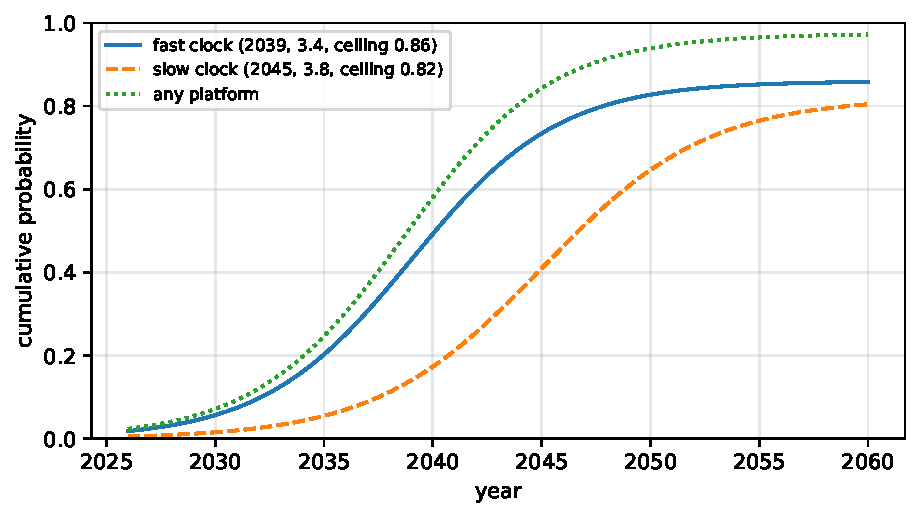
\includegraphics[width=0.82\linewidth]{figures/fig_cdfs.pdf}
\caption{Illustrative defective capability CDFs. They are scenario inputs, not estimates of real-world arrival.}
\label{fig:cdfs}
\end{figure}

The schedule experiment deliberately uses Equation~\eqref{eq:hndlsep}, not the budget-constrained $H_B$ in Equation~\eqref{eq:hndlb}. It therefore minimises $J_{\mathrm{sep}}$ from Equation~\eqref{eq:objectivesep}, restricted to future avoidable HNDL, with constant emission, unit capture scenario weight, constant value during shelf life, and the ``any platform'' CDF. Five years of pre-2026 vulnerable emission form the historical stock. The scalar benchmark sets $\alpha=\beta=1$ and omits cost because every schedule executes the same projects for the same total duration. Consequently, the reported percentage reductions apply only to the separable, unlimited-throughput exposure benchmark. They do not estimate reductions in realised compromise or in the finite-budget objective $J_B$, and a binding work budget could change the schedule ranking. Figure~\ref{fig:pareto} reports the underlying live/separable-HNDL trade-off.

Four heuristics are compared with exhaustive optimisation:

\begin{itemize}
\item criticality-first, breaking ties by live value;
\item shelf-life score, ranking by HNDL rate times shelf life;
\item live-value first;
\item shortest-job first, breaking ties by criticality.
\end{itemize}

\begin{table}[ht]
\centering
\caption{Synthetic separable-benchmark results. The total is live plus future $H_{\mathrm{sep}}$, not the finite-budget $H_B$; historical separable HNDL is invariant at 75.75 units.}
\label{tab:results}
\small
\begin{tabular}{@{}llrrrr@{}}
\toprule
Scenario & Policy & Live & Future $H_{\mathrm{sep}}$ & Benchmark total & Versus criticality \\
\midrule
Fast-first & Criticality-first & 25.07 & 160.45 & 185.52 & -- \\
 & Shelf-life score & 53.26 & 92.24 & 145.50 & $-21.6\%$ \\
 & Live-value first & 23.65 & 170.72 & 194.37 & $+4.8\%$ \\
 & Shortest-job first & 27.55 & 126.43 & 153.98 & $-17.0\%$ \\
 & Optimised & 53.60 & 78.83 & \textbf{132.43} & $\mathbf{-28.6\%}$ \\
\addlinespace
Slow-first & Criticality-first & 17.12 & 160.45 & 177.57 & -- \\
 & Shelf-life score & 29.85 & 92.24 & 122.09 & $-31.2\%$ \\
 & Live-value first & 19.25 & 170.72 & 189.98 & $+7.0\%$ \\
 & Shortest-job first & 19.98 & 126.43 & 146.42 & $-17.5\%$ \\
 & Optimised & 32.45 & 77.35 & \textbf{109.79} & $\mathbf{-38.2\%}$ \\
\bottomrule
\end{tabular}
\end{table}

The fast-first optimum is M\&A $\rightarrow$ genomics $\rightarrow$ telemetry $\rightarrow$ identity $\rightarrow$ transactions $\rightarrow$ code signing. In the slow-first case, the final two projects swap: code signing precedes transactions. This is a small but direct demonstration that platform/attack class can change a schedule even when the organisation's portfolio is unchanged.

The equal-weight separable optimum deliberately accepts more live exposure than criticality-first to reduce a much larger future $H_{\mathrm{sep}}$ term. It should not be interpreted as the $J_B$ optimum or as a recommendation to subordinate safety-critical or legally mandated controls. Those requirements belong in hard constraints or in a defensible weighting process.

\begin{figure}[ht]
\centering
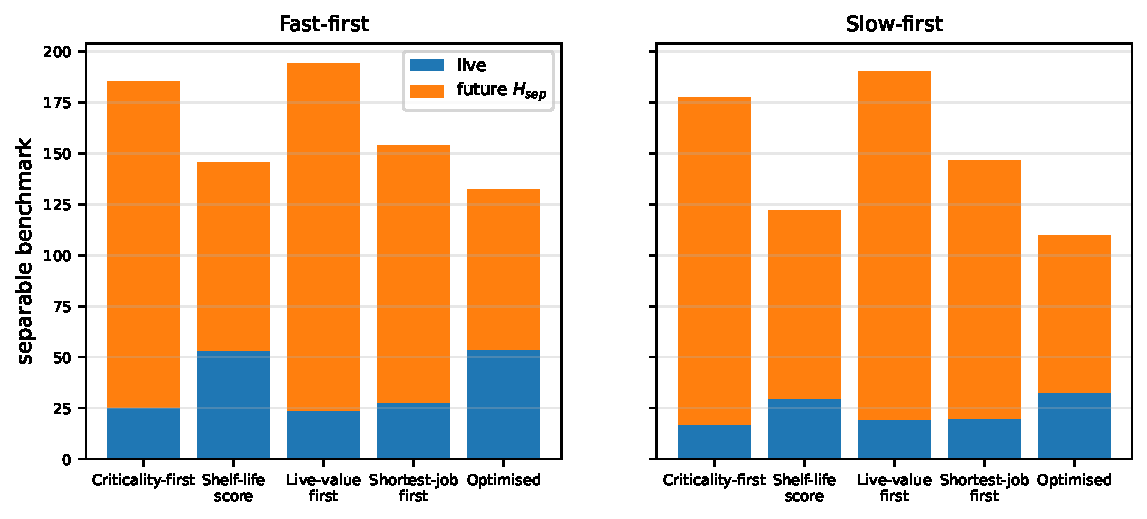
\includegraphics[width=0.88\linewidth]{figures/fig_policy_comparison.pdf}
\caption{Separable benchmark under four heuristics and exact enumeration. The plotted values use $H_{\mathrm{sep}}$, not budget-constrained $H_B$.}
\label{fig:policies}
\end{figure}

\begin{figure}[ht]
\centering
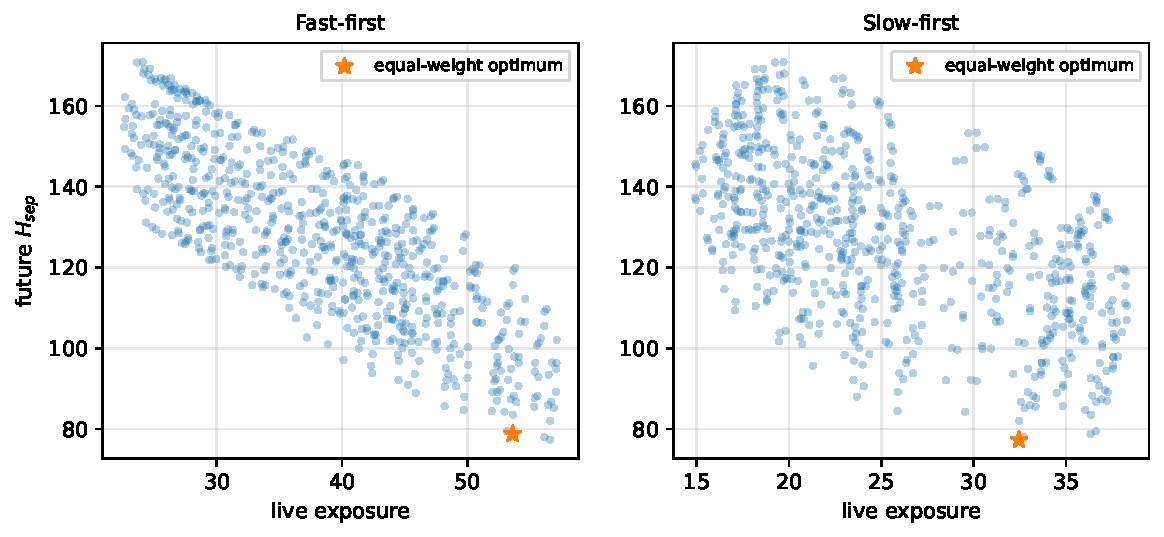
\includegraphics[width=0.88\linewidth]{figures/fig_pareto.pdf}
\caption{Every feasible schedule in live/separable-HNDL space. This is not a finite-budget $H_B$ frontier. A frontier, rather than one scalar optimum, is appropriate when governance weights are disputed.}
\label{fig:pareto}
\end{figure}

\begin{figure}[ht]
\centering
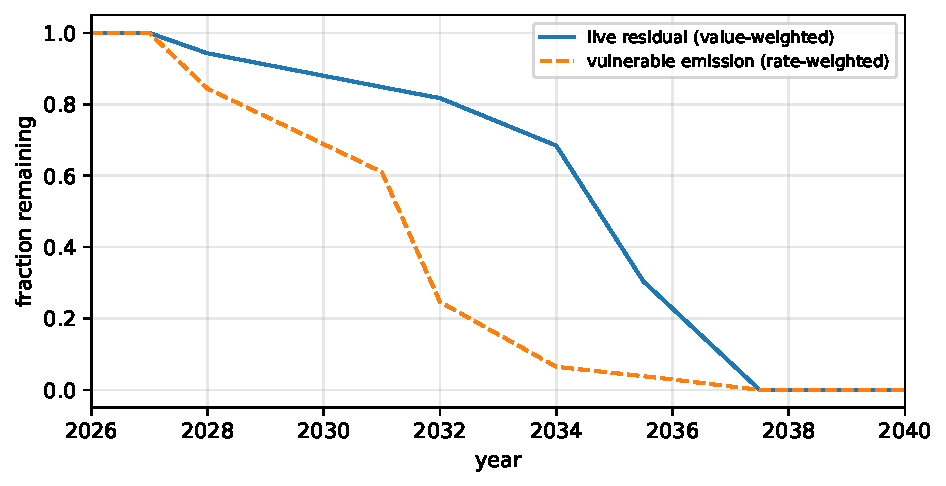
\includegraphics[width=0.84\linewidth]{figures/fig_trajectories.pdf}
\caption{Portfolio trajectories for the equal-weight separable optimum. Live residual and vulnerable emission decline differently because migration order acts on different system attributes.}
\label{fig:trajectory}
\end{figure}

\FloatBarrier

The historical HNDL component is 75.75 units in every schedule. Reporting it separately prevents a common interpretive error: a completed migration stops new vulnerable emission but does not erase a previously captured archive. Conversely, because the historical stock is invariant, it should not affect the ranking of schedules in this experiment.

\subsection{Work-budget sensitivity}

To illustrate Equation~\eqref{eq:knapsack}, we construct six archive classes with values $(40,30,24,18,12,8)$ and baseline work costs $(40,25,18,12,8,5)$. This sensitivity calculation is separate from the 720-schedule experiment and does not generate its headline percentages. Figure~\ref{fig:budget} applies global work multipliers that could represent independent rekeying or larger key-exchange parameters. At budget 60, realisable value falls from 82.4 at baseline work to 44.7 at $2\times$, 18.5 at $5\times$, and 9.5 at $10\times$. The curve is piecewise linear, not proportional, because the adversary reprioritises targets.

\begin{figure}[ht]
\centering
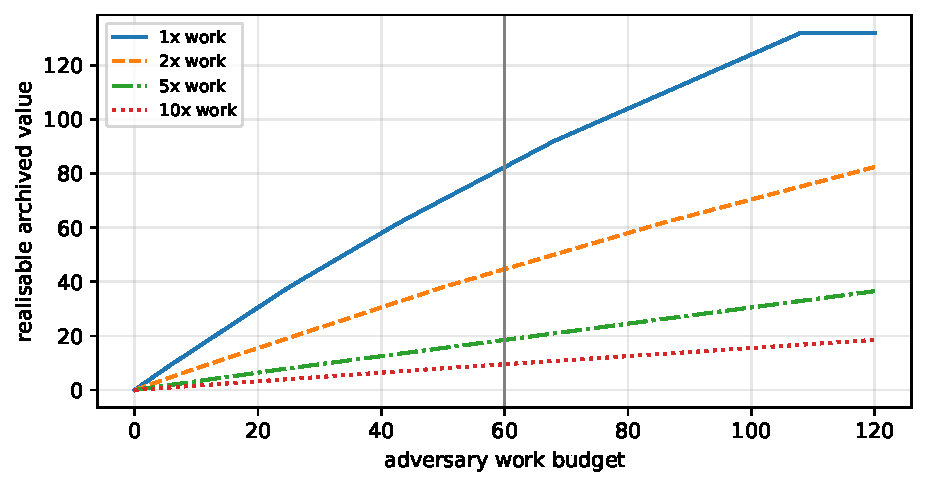
\includegraphics[width=0.82\linewidth]{figures/fig_budget.pdf}
\caption{Fractional-knapsack upper bound on realisable archived value. Increasing work per recovered unit is a control lever even before complete migration.}
\label{fig:budget}
\end{figure}

\FloatBarrier

\section{From inventory to implementation}

CCE is designed to consume, not replace, a cryptographic inventory. A minimum data schema is shown in Table~\ref{tab:schema}.

\begin{table}[ht]
\centering
\caption{Minimum auditable input schema.}
\label{tab:schema}
\small
\begin{tabularx}{\linewidth}{@{}p{0.25\linewidth}X@{}}
\toprule
Field & Required interpretation \\
\midrule
System/data-class identifier & Stable identifier linked to the cryptographic inventory and owner. \\
Security property & Confidentiality, authentication, integrity, non-repudiation, or asset control; do not collapse them. \\
Vulnerable primitive/mode & Algorithm, parameters, protocol mode, forward-secrecy and recovery-scope facts. \\
Attack class and window & At-rest, live/on-spend, on-setup, or another declared class; wall-clock threshold. \\
Residual trajectory $R_i(t;s)$ & Planned protected fraction over time, including dependencies and rollback risk. \\
Consequence unit $V_{ia}$ & Currency, records, keys, or normalised unit with conversion rationale. \\
Emission $h_i(u)$ and capture $c_i(u)$ & Measured or bounded flow and an explicitly scenario-dependent capture assumption. \\
Shelf-life/value decay & Regulatory or business retention of confidentiality, not merely storage retention. \\
Quantum work $w_{jp}(t)$ & Recovery scope and work per independently protected object/epoch. \\
Evidence provenance & Source, version, date, confidence interval, and update rule for each parameter. \\
\bottomrule
\end{tabularx}
\end{table}

A deployment workflow is:

\begin{enumerate}
\item define operational capability classes before choosing timelines;
\item map cryptographic dependencies and data classes;
\item elicit ranges for consequence, emission, shelf life, and capture scenarios;
\item build platform-conditioned $F_{pa}$ as scenario ensembles, preserving disagreement rather than averaging it away;
\item generate feasible migration trajectories from resource and dependency constraints;
\item compute Pareto frontiers and sensitivity to every contested input;
\item freeze evidence and policy weights for each decision record;
\item update distributions only through a pre-declared evidence process.
\end{enumerate}

The output should include component exposures, not only $J_B(s)$ or $J_{\mathrm{sep}}(s)$. Decision-makers must be able to see whether an apparently good schedule buys HNDL reduction by accepting live exposure, as in the synthetic example.

\section{Validation and falsification programme}

The framework is mathematically defined, but its practical validity depends on inputs. A defensible empirical programme should test the following.

\paragraph{Construct validity.} Compare CCE rankings with independent expert pairwise judgements after experts receive the same inventory. Disagreement should be traced to inputs or utility weights rather than hidden scoring rules.

\paragraph{Predictive process validity.} In organisations with multi-year migration records, compare planned $R_i(t;s)$ with realised trajectories and estimate schedule slippage distributions. The model should be recalculated using realised paths.

\paragraph{Sensitivity and value of information.} Report rank stability under alternative $F_{pa}$, capture probabilities, shelf-life bounds, and consequence weights. Inputs whose uncertainty changes the Pareto set are candidates for measurement; inputs that do not change decisions should not receive false precision.

\paragraph{HNDL work calibration.} Map protocol configurations to recovery scope and quantum work. Static RSA key transport, ephemeral ECDHE, TLS resumption chains, SSH rekey epochs, and future hybrid modes must not share one $w_j$ \cite{blanco2026}.

\paragraph{Platform calibration.} A platform-conditioned capability distribution should respond to resource-estimate revisions, demonstrated error-correction cycles, throughput, decoding/control limitations, and endurance evidence. It should not respond directly to marketing roadmaps without a declared likelihood model.

\paragraph{Evidence-channel calibration.} Before using blockchain anomalies for updating, backtest the monitor on historical dormant-key movement and known classical compromises. Publish false-positive rates and avoid address-level target lists when cohort aggregates suffice.

CCE would be practically falsified as a useful decision aid if, across diverse realistic inputs, its ranking collapses to an existing simpler rule without material loss; if organisations cannot supply bounds tight enough to stabilise decisions; or if migration trajectories are too endogenous for prospective use. Those are empirical questions, not matters of branding.

\section{Limitations and threats to validity}

\begin{enumerate}
\item \textbf{Arrival distributions are beliefs, not frequencies.} Expert surveys and hardware models disagree, and covert capability is unobservable. Defective distributions and scenario ensembles make this visible but do not remove epistemic uncertainty.
\item \textbf{Platform classes are coarse.} Fast-clock and slow-clock are useful attack-window categories, not immutable physical laws. Photonic, silicon-spin, superconducting, neutral-atom, and ion-trap systems have heterogeneous scaling constraints.
\item \textbf{Exposure is not loss.} Equation~\eqref{eq:live} omits adversary intent, target choice, exploit operationalisation, controls outside cryptography, and loss-given-compromise unless users explicitly add them.
\item \textbf{Shelf life is difficult to elicit.} Regulatory retention can bound storage duration but not always the future value of disclosure. Value decay may be non-linear and event-dependent.
\item \textbf{Capture is rarely observed.} HNDL capture probability is a scenario parameter. Treating all traffic as captured is a stress test, not a factual claim.
\item \textbf{The case study is synthetic and uses the separable benchmark.} The reported percentage improvements are not external validation, must not be reused as industry estimates, and are not estimates of improvement under finite-budget $H_B$. The isolated work-budget sensitivity does not establish that the same schedules remain optimal when the budget binds.
\item \textbf{Scalarisation embeds policy.} Equal weights in the experiment are arbitrary. Safety, legal, and fiduciary constraints may dominate any exposure calculation.
\item \textbf{Prior-art search is not a systematic review.} Search-engine coverage, terminology, paywalls, and unpublished consultancy methods limit the novelty assessment. The strongest defensible claim is ``not found in the retrieved corpus,'' not ``does not exist.''
\item \textbf{Correlated arrivals and common causes matter.} The independent platform CDF combination used in the experiment is illustrative. Real forecasts require a joint model because algorithmic advances and error-correction breakthroughs affect multiple platforms.
\item \textbf{Migration can create risk.} Hybrid deployment, certificate expansion, protocol fallback, implementation flaws, and operational outages belong in $C(s)$ or constraints and require separate security analysis \cite{hasan2024}.
\end{enumerate}

\section{Discussion}

The main conceptual change is modest: replace a date or score with a trajectory evaluated against a distribution. Its consequences are less modest.

First, uncertainty can become operationally useful. A model need not publish a median Q-Day to compare schedules. It can integrate over an entire censored scenario ensemble. Second, HNDL is not simply ``on'' until migration. Its future component depends on emission, lifetime, capture, recovery scope, and finite work. Third, platform class matters because capability is attack-specific. A system exposed only during a short live window should not be evaluated against the same arrival event as a long-lived archive. Fourth, past HNDL exposure and future preventable flow should be shown separately: one measures inherited liability; the other measures what the current programme can still change.

This framing also clarifies the role of endurance research. Correlated radiation events in superconducting hardware may affect the cost or time at which a reliable fast-clock cryptanalytic capability exists. They do not, without additional evidence, prove infeasibility or yield a direct logical error multiplier. The correct interface between literatures is a platform-conditioned capability distribution with traceable assumptions.

Finally, a live evidence channel is useful only if it respects causal ambiguity. Several unrelated old keys moving in a short window could be informative; it could also indicate a classical common-mode compromise. The scientific product is a baseline, anomaly statistic, and update rule, not an alarm headline.

\section{Conclusion}

Post-quantum migration is a scheduling decision under deep uncertainty. A deadline states when a transition should finish; a readiness score describes present state; an inventory lists what exists. None alone answers how much consequence-weighted vulnerability will remain when a specified cryptanalytic capability first becomes available, or how much valuable ciphertext will have accumulated by then.

Capability-conditioned exposure supplies that missing link. It evaluates residual migration trajectories against attack- and platform-specific arrival distributions, separates live from HNDL exposure, recognises the sunk stock of previously captured ciphertext, and constrains future decryption by quantum work. The framework is intentionally transparent about what it cannot infer. Its value is not a more dramatic Q-Day claim, but a reproducible way to compare actions without pretending the date is known.

The synthetic case study shows that combining capability-conditioned live exposure with the separable future-HNDL benchmark can change migration order and that criticality-first can be materially suboptimal under declared assumptions. It does not numerically test the finite-budget objective $J_B$; the knapsack mechanism is demonstrated separately. The next research step is not a larger synthetic score. It is a preregistered empirical study using anonymised cryptographic inventories, bounded data-lifetime inputs, realised migration trajectories, and multiple independently constructed capability distributions.

\appendix
\section{Reproduction notes}

The accompanying script \texttt{analysis\_model.py} uses Python and Matplotlib. It defines every
synthetic input, enumerates all 720 schedules, writes machine-readable inputs and results, and
recreates all figures. No random sampling is used, so results are deterministic subject to
ordinary floating-point differences. Every figure in this paper and every number in
Table~\ref{tab:results}, the historical component, and the budget curve are produced
by that one script; nothing is transcribed by hand.

For each scenario, live exposure is evaluated by discrete Stieltjes increments on a half-month grid from 2026 to 2060. Future $H_{\mathrm{sep}}$ is integrated on the same grid. Historical separable HNDL covers 2021 to 2026. Exhaustive enumeration chooses the minimum of live plus future $H_{\mathrm{sep}}$; historical HNDL is reported but excluded from schedule comparison because it is invariant. The script does not feed the separate fractional-knapsack sensitivity into schedule enumeration.

\section{Additional interpretation rules}

\begin{itemize}
\item Never compare CCE values across organisations unless units, boundaries, capability definitions, and weights are identical.
\item Never describe normalised exposure units as probability, currency, or expected loss.
\item Never infer a quantum cause from a ledger anomaly without an explicit competing-cause model.
\item Never map a physical radiation impact rate directly to a logical cryptanalytic failure rate.
\item Never combine platform CDFs as independent without marking independence as an assumption.
\item Always publish the historical HNDL stock separately from future avoidable flow.
\item Prefer Pareto frontiers when live exposure, confidentiality exposure, cost, and safety cannot be placed in one defensible unit.
\end{itemize}

\section{Prior-art search log}

The search was executed on 13 August 2026 and covered records available up to that date. Sources were IACR ePrint, arXiv, NIST/NCCoE, ETSI, discoverable IEEE metadata, and general web search used to locate practitioner frameworks. Representative queries were:

\begin{itemize}
\item \texttt{"post-quantum" migration risk "arrival distribution"};
\item \texttt{"data shelf life" quantum risk migration};
\item \texttt{HNDL economic quantum work rekeying};
\item \texttt{post-quantum migration schedule optimization};
\item \texttt{platform fast-clock slow-clock quantum cryptanalysis};
\item \texttt{cryptographic exposure trajectory quantum}; and
\item site-restricted variants for \texttt{eprint.iacr.org}, \texttt{arxiv.org}, \texttt{nist.gov}, and \texttt{etsi.org}.
\end{itemize}

Works were retained when they supplied at least one of: a migration decision model, a quantum-arrival distribution, an HNDL cost or lifetime model, an attack-window/platform distinction, or hardware evidence affecting effective cryptanalytic capability. Pure PQC performance benchmarks were excluded unless they directly modelled migration or exposure. Backward citation chasing was applied to the closest retained works. Search results and commercial material were used for discovery; technical claims were traced to primary papers or official standards where available. This protocol is reproducible in intent but is not PRISMA-complete and does not support a claim of exhaustive novelty.

\section{Author contributions and tool use}

The framework, the analysis and the manuscript were developed with substantial assistance from large language model tooling, used for literature retrieval, drafting, derivation checking and revision. All cited sources were traced to their primary records. The author takes full responsibility for the content, the claims, and the verification of every reference.

\begin{thebibliography}{99}
\small

\bibitem{shor1994}
P. W. Shor, ``Algorithms for quantum computation: discrete logarithms and factoring,'' in \emph{Proceedings of the 35th Annual Symposium on Foundations of Computer Science}, 1994, pp. 124--134.

\bibitem{mosca2018}
M. Mosca, ``Cybersecurity in an era with quantum computers: Will we be ready?'' \emph{IEEE Security \& Privacy}, vol. 16, no. 5, pp. 38--41, 2018. doi: \href{https://doi.org/10.1109/MSP.2018.3761723}{10.1109/MSP.2018.3761723}.

\bibitem{nistpqc}
National Institute of Standards and Technology, ``Post-Quantum Cryptography Project,'' updated 5 August 2026. \url{https://csrc.nist.gov/projects/post-quantum-cryptography}.

\bibitem{nist8547}
D. Moody, R. Perlner, A. Regenscheid, A. Robinson, and D. Cooper, \emph{Transition to Post-Quantum Cryptography Standards}, NIST IR 8547 Initial Public Draft, 2024. doi: \href{https://doi.org/10.6028/NIST.IR.8547.ipd}{10.6028/NIST.IR.8547.ipd}.

\bibitem{nccoe}
National Cybersecurity Center of Excellence, ``Migration to Post-Quantum Cryptography,'' 2026. \url{https://www.nccoe.nist.gov/applied-cryptography/migration-to-pqc}.

\bibitem{etsi}
ETSI, \emph{Quantum Safe Cryptography; Quantum-Safe Threat Assessment}, ETSI GR QSC 004 V1.1.1, 2017. \url{https://www.etsi.org/deliver/etsi_gr/QSC/001_099/004/01.01.01_60/gr_QSC004v010101p.pdf}.

\bibitem{gri2025}
M. Mosca and M. Piani, \emph{Quantum Threat Timeline Report 2025}, Global Risk Institute and evolutionQ, 2026. \url{https://globalriskinstitute.org/publication/2025-quantum-threat-timeline-report/}.

\bibitem{hasan2024}
K. F. Hasan et al., ``A framework for migrating to post-quantum cryptography: Security dependency analysis and case studies,'' \emph{IEEE Access}, vol. 12, pp. 23427--23450, 2024. doi: \href{https://doi.org/10.1109/ACCESS.2024.3360412}{10.1109/ACCESS.2024.3360412}.

\bibitem{chammas2026}
P. Chammas, K. Hariss, C. Bassil, and M. Chamoun, ``Towards a field-informed risk-based framework for PQC migration in legacy systems,'' IACR Cryptology ePrint Archive, Paper 2026/790, 2026. \url{https://eprint.iacr.org/2026/790}.

\bibitem{cars2026}
A. D. B. Costa, ``Quantum-safe cryptography: A migration framework for legacy systems toward NIST PQC standards with the Crypto-Agility Readiness Score,'' IACR Cryptology ePrint Archive, Paper 2026/1467, 2026. \url{https://eprint.iacr.org/2026/1467}.

\bibitem{tlsrisk2026}
Y.-L. Hyoung et al., ``A layered risk scoring model for TLS connections against quantum threats,'' IACR Cryptology ePrint Archive, Paper 2026/1174, 2026. \url{https://eprint.iacr.org/2026/1174}.

\bibitem{blanco2026}
J. Blanco-Romero, F. Almenares Mendoza, C. Garc\'ia Rubio, C. Campo, and D. D\'iaz S\'anchez, ``On the practical feasibility of harvest-now, decrypt-later attacks,'' arXiv:2603.01091, 2026. \url{https://arxiv.org/abs/2603.01091}.

\bibitem{sammo2026}
N. S. Sammo, ``Post-quantum cryptography migration in Australian real-time payment infrastructure: A Monte Carlo simulation study of the New Payments Platform,'' arXiv:2605.02276, 2026. \url{https://arxiv.org/abs/2605.02276}.

\bibitem{horizon2026}
I. M. Gershteyn and J. A. Alber, ``Quantum Horizon: An evaluation of quantum computing as a threat to Bitcoin and Ethereum,'' arXiv:2606.14484, 2026. \url{https://arxiv.org/abs/2606.14484}.

\bibitem{babbush2026}
R. Babbush et al., ``Securing elliptic curve cryptocurrencies against quantum vulnerabilities: Resource estimates and mitigations,'' IACR Cryptology ePrint Archive, Paper 2026/625, 2026. \url{https://eprint.iacr.org/2026/625}.

\bibitem{mcewen2021}
M. McEwen et al., ``Resolving catastrophic error bursts from cosmic rays in large arrays of superconducting qubits,'' \emph{Nature Physics}, vol. 18, pp. 107--111, 2022; arXiv:2104.05219. \url{https://arxiv.org/abs/2104.05219}.

\bibitem{q3de2025}
Y. Suzuki, T. Sugiyama, T. Arai, W. Liao, K. Inoue, and T. Tanimoto, ``Q3DE: A fault-tolerant quantum computer architecture for multi-bit burst errors by cosmic rays,'' arXiv:2501.00331, 2025. \url{https://arxiv.org/abs/2501.00331}.

\bibitem{nho2026}
H. Nho et al., ``Recovery dynamics of a gap-engineered transmon after a quasiparticle burst,'' \emph{Physical Review Letters}, vol. 136, 050601, 2026; arXiv:2505.08104. \url{https://arxiv.org/abs/2505.08104}.

\bibitem{pinckney2026}
H. D. Pinckney et al., ``Characterization of radiation-induced errors in superconducting qubits protected with various gap-engineering strategies,'' arXiv:2603.13460, 2026. \url{https://arxiv.org/abs/2603.13460}.

\bibitem{cain2026}
M. Cain, Q. Xu, R. King, L. R. B. Picard et al., ``Shor's algorithm is possible with as few as 10,000 reconfigurable atomic qubits,'' arXiv:2603.28627, 2026. \url{https://arxiv.org/abs/2603.28627}.

\bibitem{pinnacle2026}
``The Pinnacle Architecture: Reducing the cost of breaking RSA-2048 to 100\,000 physical qubits using quantum LDPC codes,'' arXiv:2602.11457, 2026. \url{https://arxiv.org/abs/2602.11457}.

\bibitem{conceptualise2026}
CC Conceptualise GmbH, ``Harvest Now, Decrypt Later: The Quantum Data Risk Model,'' 31 May 2026. \url{https://www.conceptualise.de/en/blog/harvest-now-decrypt-later-risk-model}. Practitioner source; not peer reviewed.

\bibitem{applied2026}
M. Ivezic and Applied Quantum, \emph{The Applied Quantum PQC Migration Framework and Methodology}, version 2.1, June 2026. \url{https://pqcframework.com/}. Practitioner framework; not peer reviewed.

\end{thebibliography}

\end{document}
